% Options for packages loaded elsewhere
\PassOptionsToPackage{unicode}{hyperref}
\PassOptionsToPackage{hyphens}{url}
%
\documentclass[
]{article}
\usepackage{lmodern}
\usepackage{amssymb,amsmath}
\usepackage{ifxetex,ifluatex}
\ifnum 0\ifxetex 1\fi\ifluatex 1\fi=0 % if pdftex
  \usepackage[T1]{fontenc}
  \usepackage[utf8]{inputenc}
  \usepackage{textcomp} % provide euro and other symbols
\else % if luatex or xetex
  \usepackage{unicode-math}
  \defaultfontfeatures{Scale=MatchLowercase}
  \defaultfontfeatures[\rmfamily]{Ligatures=TeX,Scale=1}
\fi
% Use upquote if available, for straight quotes in verbatim environments
\IfFileExists{upquote.sty}{\usepackage{upquote}}{}
\IfFileExists{microtype.sty}{% use microtype if available
  \usepackage[]{microtype}
  \UseMicrotypeSet[protrusion]{basicmath} % disable protrusion for tt fonts
}{}
\makeatletter
\@ifundefined{KOMAClassName}{% if non-KOMA class
  \IfFileExists{parskip.sty}{%
    \usepackage{parskip}
  }{% else
    \setlength{\parindent}{0pt}
    \setlength{\parskip}{6pt plus 2pt minus 1pt}}
}{% if KOMA class
  \KOMAoptions{parskip=half}}
\makeatother
\usepackage{xcolor}
\IfFileExists{xurl.sty}{\usepackage{xurl}}{} % add URL line breaks if available
\IfFileExists{bookmark.sty}{\usepackage{bookmark}}{\usepackage{hyperref}}
\hypersetup{
  pdftitle={Peer-graded Assignment: Course Project 1},
  pdfauthor={Teo Lo Piparo},
  hidelinks,
  pdfcreator={LaTeX via pandoc}}
\urlstyle{same} % disable monospaced font for URLs
\usepackage[margin=1in]{geometry}
\usepackage{color}
\usepackage{fancyvrb}
\newcommand{\VerbBar}{|}
\newcommand{\VERB}{\Verb[commandchars=\\\{\}]}
\DefineVerbatimEnvironment{Highlighting}{Verbatim}{commandchars=\\\{\}}
% Add ',fontsize=\small' for more characters per line
\usepackage{framed}
\definecolor{shadecolor}{RGB}{248,248,248}
\newenvironment{Shaded}{\begin{snugshade}}{\end{snugshade}}
\newcommand{\AlertTok}[1]{\textcolor[rgb]{0.94,0.16,0.16}{#1}}
\newcommand{\AnnotationTok}[1]{\textcolor[rgb]{0.56,0.35,0.01}{\textbf{\textit{#1}}}}
\newcommand{\AttributeTok}[1]{\textcolor[rgb]{0.77,0.63,0.00}{#1}}
\newcommand{\BaseNTok}[1]{\textcolor[rgb]{0.00,0.00,0.81}{#1}}
\newcommand{\BuiltInTok}[1]{#1}
\newcommand{\CharTok}[1]{\textcolor[rgb]{0.31,0.60,0.02}{#1}}
\newcommand{\CommentTok}[1]{\textcolor[rgb]{0.56,0.35,0.01}{\textit{#1}}}
\newcommand{\CommentVarTok}[1]{\textcolor[rgb]{0.56,0.35,0.01}{\textbf{\textit{#1}}}}
\newcommand{\ConstantTok}[1]{\textcolor[rgb]{0.00,0.00,0.00}{#1}}
\newcommand{\ControlFlowTok}[1]{\textcolor[rgb]{0.13,0.29,0.53}{\textbf{#1}}}
\newcommand{\DataTypeTok}[1]{\textcolor[rgb]{0.13,0.29,0.53}{#1}}
\newcommand{\DecValTok}[1]{\textcolor[rgb]{0.00,0.00,0.81}{#1}}
\newcommand{\DocumentationTok}[1]{\textcolor[rgb]{0.56,0.35,0.01}{\textbf{\textit{#1}}}}
\newcommand{\ErrorTok}[1]{\textcolor[rgb]{0.64,0.00,0.00}{\textbf{#1}}}
\newcommand{\ExtensionTok}[1]{#1}
\newcommand{\FloatTok}[1]{\textcolor[rgb]{0.00,0.00,0.81}{#1}}
\newcommand{\FunctionTok}[1]{\textcolor[rgb]{0.00,0.00,0.00}{#1}}
\newcommand{\ImportTok}[1]{#1}
\newcommand{\InformationTok}[1]{\textcolor[rgb]{0.56,0.35,0.01}{\textbf{\textit{#1}}}}
\newcommand{\KeywordTok}[1]{\textcolor[rgb]{0.13,0.29,0.53}{\textbf{#1}}}
\newcommand{\NormalTok}[1]{#1}
\newcommand{\OperatorTok}[1]{\textcolor[rgb]{0.81,0.36,0.00}{\textbf{#1}}}
\newcommand{\OtherTok}[1]{\textcolor[rgb]{0.56,0.35,0.01}{#1}}
\newcommand{\PreprocessorTok}[1]{\textcolor[rgb]{0.56,0.35,0.01}{\textit{#1}}}
\newcommand{\RegionMarkerTok}[1]{#1}
\newcommand{\SpecialCharTok}[1]{\textcolor[rgb]{0.00,0.00,0.00}{#1}}
\newcommand{\SpecialStringTok}[1]{\textcolor[rgb]{0.31,0.60,0.02}{#1}}
\newcommand{\StringTok}[1]{\textcolor[rgb]{0.31,0.60,0.02}{#1}}
\newcommand{\VariableTok}[1]{\textcolor[rgb]{0.00,0.00,0.00}{#1}}
\newcommand{\VerbatimStringTok}[1]{\textcolor[rgb]{0.31,0.60,0.02}{#1}}
\newcommand{\WarningTok}[1]{\textcolor[rgb]{0.56,0.35,0.01}{\textbf{\textit{#1}}}}
\usepackage{graphicx,grffile}
\makeatletter
\def\maxwidth{\ifdim\Gin@nat@width>\linewidth\linewidth\else\Gin@nat@width\fi}
\def\maxheight{\ifdim\Gin@nat@height>\textheight\textheight\else\Gin@nat@height\fi}
\makeatother
% Scale images if necessary, so that they will not overflow the page
% margins by default, and it is still possible to overwrite the defaults
% using explicit options in \includegraphics[width, height, ...]{}
\setkeys{Gin}{width=\maxwidth,height=\maxheight,keepaspectratio}
% Set default figure placement to htbp
\makeatletter
\def\fps@figure{htbp}
\makeatother
\setlength{\emergencystretch}{3em} % prevent overfull lines
\providecommand{\tightlist}{%
  \setlength{\itemsep}{0pt}\setlength{\parskip}{0pt}}
\setcounter{secnumdepth}{-\maxdimen} % remove section numbering

\title{Peer-graded Assignment: Course Project 1}
\usepackage{etoolbox}
\makeatletter
\providecommand{\subtitle}[1]{% add subtitle to \maketitle
  \apptocmd{\@title}{\par {\large #1 \par}}{}{}
}
\makeatother
\subtitle{PA1\_template.Rmd}
\author{Teo Lo Piparo}
\date{}

\begin{document}
\maketitle

\hypertarget{introduction}{%
\paragraph{Introduction}\label{introduction}}

It is now possible to collect a large amount of data about personal
movement using activity monitoring devices such as a
\href{http://www.fitbit.com/}{Fitbit},
\href{http://www.nike.com/us/en_us/c/nikeplus-fuelband}{Nike Fuelband},
or \href{https://jawbone.com/up}{Jawbone Up}. These type of devices are
part of the ``quantified self'' movement -- a group of enthusiasts who
take measurements about themselves regularly to improve their health, to
find patterns in their behavior, or because they are tech geeks. But
these data remain under-utilized both because the raw data are hard to
obtain and there is a lack of statistical methods and software for
processing and interpreting the data.

This assignment makes use of data from a personal activity monitoring
device. This device collects data at 5 minute intervals through out the
day. The data consists of two months of data from an anonymous
individual collected during the months of October and November, 2012 and
include the number of steps taken in 5 minute intervals each day.

The data for this assignment can be downloaded from the course web site:

Dataset:
\href{https://d396qusza40orc.cloudfront.net/repdata\%2Fdata\%2Factivity.zip}{Activity
monitoring data} {[}52K{]}

\textbf{The variables included in this dataset are:}

\begin{itemize}
\tightlist
\item
  \texttt{steps}: Number of steps taking in a 5-minute interval (missing
  values are coded as \color{red}{\verb|NA|}NA)
\item
  \texttt{date}: The date on which the measurement was taken in
  \texttt{YYYY-MM-DD} format
\item
  \texttt{interval}: Identifier for the 5-minute interval in which
  measurement was taken
\end{itemize}

The dataset is stored in a comma-separated-value (CSV) file and there
are a total of 17,568 observations in this dataset.

\hypertarget{loading-and-preprocessing-the-data}{%
\subsubsection{Loading and preprocessing the
data}\label{loading-and-preprocessing-the-data}}

\begin{itemize}
\tightlist
\item
  Load the data (i.e.~\color{red}{\verb|read.csv()|}\texttt{read.csv()})
\item
  Process/transform the data (if necessary) into a format suitable for
  your analysis
\end{itemize}

\begin{Shaded}
\begin{Highlighting}[]
\KeywordTok{library}\NormalTok{(ggplot2)}
\KeywordTok{library}\NormalTok{(data.table)}
\KeywordTok{library}\NormalTok{(lubridate)}
\KeywordTok{library}\NormalTok{(dplyr)}
\KeywordTok{library}\NormalTok{(lattice)}
\KeywordTok{library}\NormalTok{(gridExtra)}

\NormalTok{fileUrl <-}
\StringTok{    "https://d396qusza40orc.cloudfront.net/repdata%2Fdata%2Factivity.zip"}
\KeywordTok{download.file}\NormalTok{(fileUrl, }\DataTypeTok{destfile =} \StringTok{"./repdata%2Fdata%2Factivity.zip"}\NormalTok{, }\DataTypeTok{mode =} \StringTok{"wb"}\NormalTok{)}
\CommentTok{## Unzip file}
\KeywordTok{unzip}\NormalTok{(}
    \StringTok{"./repdata%2Fdata%2Factivity.zip"}\NormalTok{,}
    \DataTypeTok{exdir =} \StringTok{"./Unzipped"}
\NormalTok{)}
\CommentTok{## Read File}
\NormalTok{csv0 <-}\StringTok{ }\KeywordTok{read.csv}\NormalTok{(}\StringTok{"./Unzipped/activity.csv"}\NormalTok{, }\DataTypeTok{header =} \OtherTok{TRUE}\NormalTok{, }\DataTypeTok{sep =} \StringTok{","}\NormalTok{)}
\KeywordTok{str}\NormalTok{(}\KeywordTok{head}\NormalTok{(csv0))}
\end{Highlighting}
\end{Shaded}

\begin{verbatim}
## 'data.frame':    6 obs. of  3 variables:
##  $ steps   : int  NA NA NA NA NA NA
##  $ date    : chr  "2012-10-01" "2012-10-01" "2012-10-01" "2012-10-01" ...
##  $ interval: int  0 5 10 15 20 25
\end{verbatim}

\hypertarget{what-is-mean-total-number-of-steps-taken-per-day}{%
\subsubsection{What is mean total number of steps taken per
day?}\label{what-is-mean-total-number-of-steps-taken-per-day}}

\textbf{For this part of the assignment, you can ignore the missing
values in the dataset.}

\begin{itemize}
\tightlist
\item
  Calculate the total number of steps taken per day.
\end{itemize}

\begin{Shaded}
\begin{Highlighting}[]
\KeywordTok{Sys.setlocale}\NormalTok{(}\StringTok{"LC_ALL"}\NormalTok{, }\StringTok{"English"}\NormalTok{)}
\end{Highlighting}
\end{Shaded}

\begin{verbatim}
## [1] "LC_COLLATE=English_United States.1252;LC_CTYPE=English_United States.1252;LC_MONETARY=English_United States.1252;LC_NUMERIC=C;LC_TIME=English_United States.1252"
\end{verbatim}

\begin{Shaded}
\begin{Highlighting}[]
\NormalTok{step0 <-}\StringTok{ }\KeywordTok{aggregate}\NormalTok{(steps}\OperatorTok{~}\NormalTok{.,}\DataTypeTok{data =}\NormalTok{ csv0, sum)}
\NormalTok{step0 <-}\StringTok{ }\NormalTok{step0[,}\KeywordTok{c}\NormalTok{(}\DecValTok{1}\NormalTok{,}\DecValTok{3}\NormalTok{)] ; }
\NormalTok{step0[,}\DecValTok{1}\NormalTok{] <-}\StringTok{ }\KeywordTok{as.Date}\NormalTok{(step0}\OperatorTok{$}\NormalTok{date)}
\end{Highlighting}
\end{Shaded}

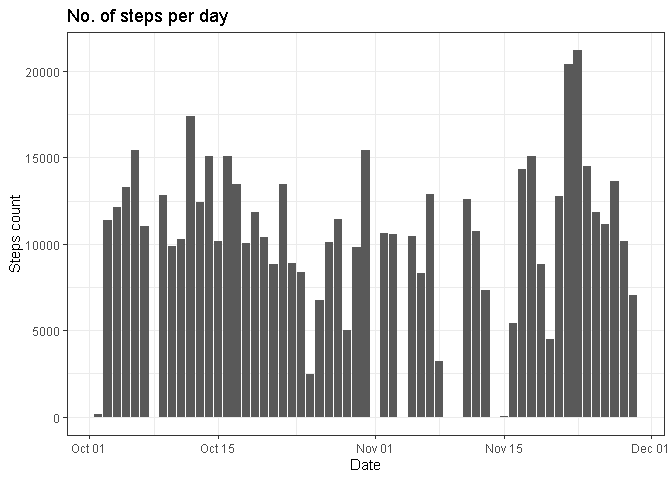
\includegraphics{PA1_template_files/figure-latex/unnamed-chunk-3-1.pdf}

\textbf{If you do not understand the difference between a histogram and
a barplot, research the difference between them. Make a histogram of the
total number of steps taken each day.}

\begin{itemize}
\tightlist
\item
  Calculate and report the mean and median of the total number of steps
  taken per day
\end{itemize}

\begin{Shaded}
\begin{Highlighting}[]
\NormalTok{step1 <-}\StringTok{ }\KeywordTok{aggregate}\NormalTok{(steps }\OperatorTok{~}\StringTok{ }\NormalTok{., }\DataTypeTok{data =}\NormalTok{ step0, mean)}
\NormalTok{step2 <-}\StringTok{ }\KeywordTok{median}\NormalTok{(step1[,}\DecValTok{2}\NormalTok{],}\DataTypeTok{na.rm =}\NormalTok{ T)}
\end{Highlighting}
\end{Shaded}

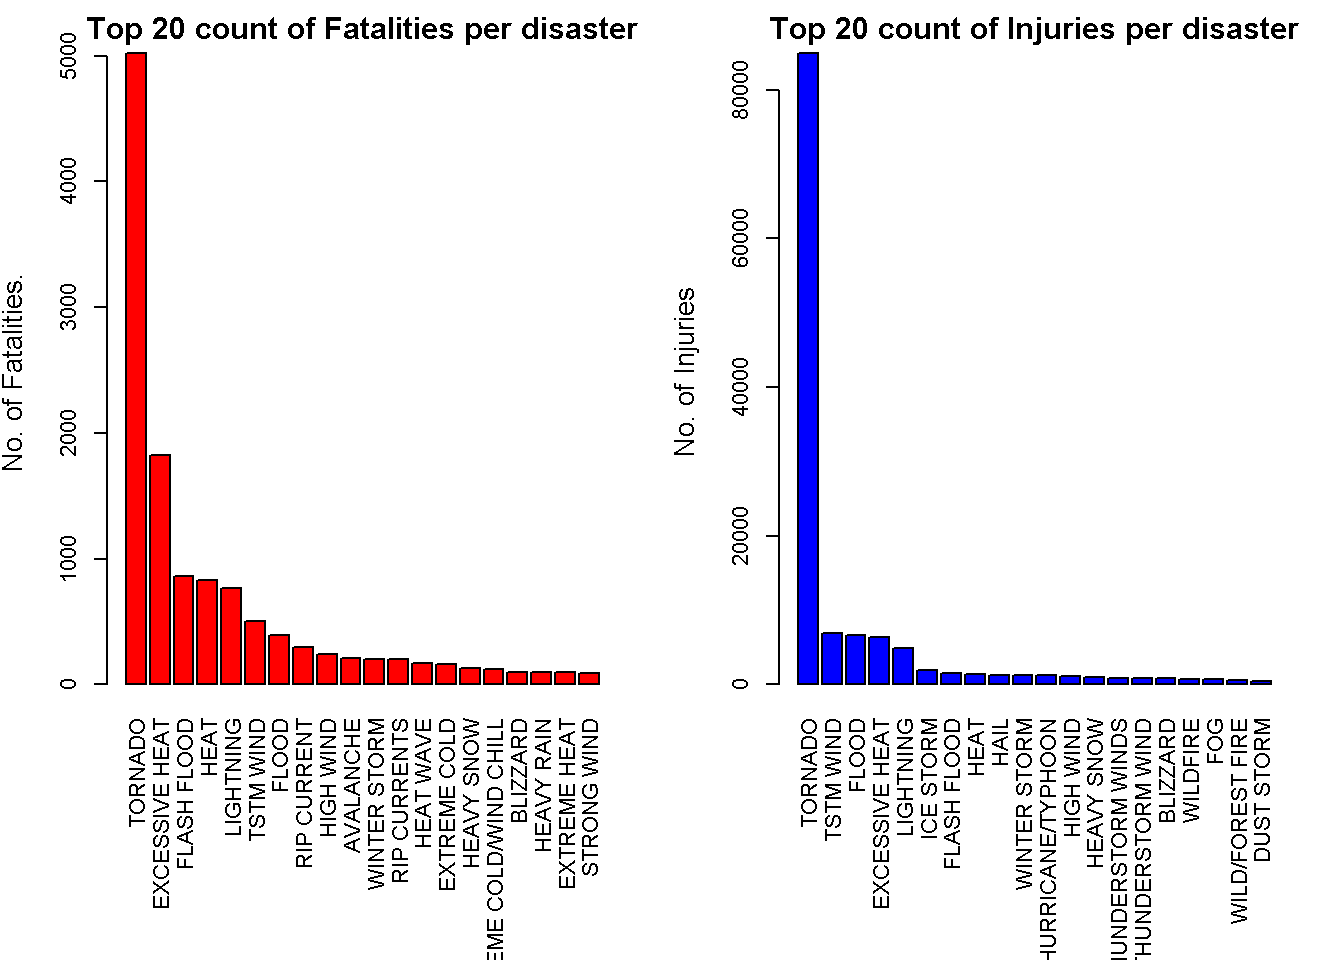
\includegraphics{PA1_template_files/figure-latex/unnamed-chunk-5-1.pdf}

\hypertarget{what-is-the-average-daily-activity-pattern}{%
\subsubsection{What is the average daily activity
pattern?}\label{what-is-the-average-daily-activity-pattern}}

\begin{itemize}
\tightlist
\item
  Make a time series plot
  (i.e.~\color{red}{\verb|type = "l"|}\texttt{type\ =\ "l"}) of the
  5-minute interval (x-axis) and the average number of steps taken,
  averaged across all days (y-axis).
\end{itemize}

\begin{Shaded}
\begin{Highlighting}[]
\NormalTok{step3 <-}\StringTok{ }\KeywordTok{aggregate}\NormalTok{(steps }\OperatorTok{~}\StringTok{ }\NormalTok{interval, }\DataTypeTok{data =}\NormalTok{ csv0, mean)}
\NormalTok{step4 <-}\StringTok{ }\KeywordTok{aggregate}\NormalTok{(steps }\OperatorTok{~}\StringTok{ }\NormalTok{date, }\DataTypeTok{data =}\NormalTok{ csv0, mean)}
\end{Highlighting}
\end{Shaded}

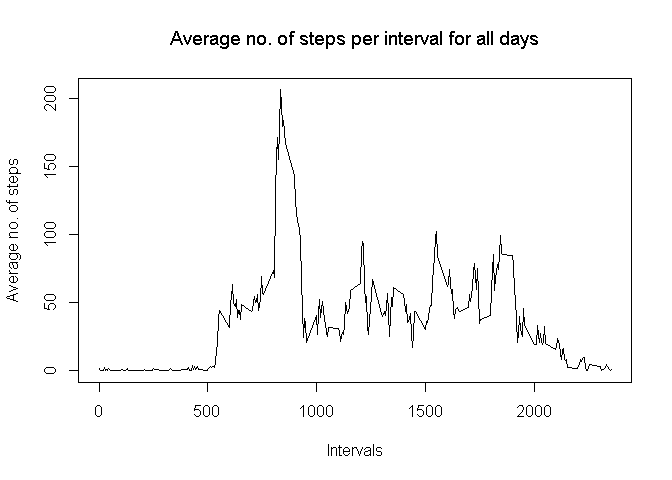
\includegraphics{PA1_template_files/figure-latex/unnamed-chunk-7-1.pdf}

\textbf{Another way of answering the above question:}

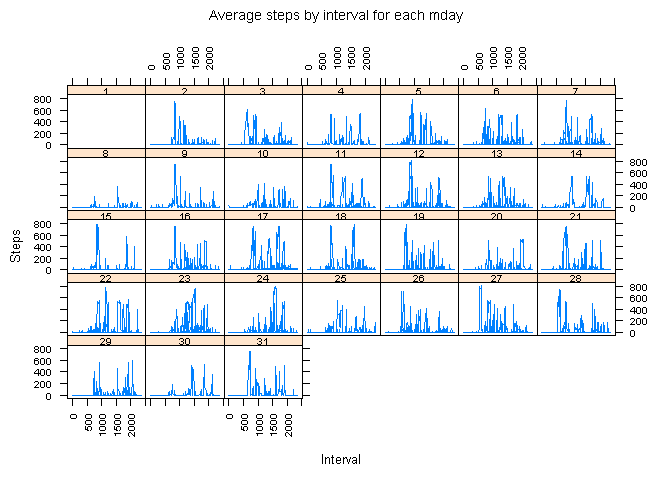
\includegraphics{PA1_template_files/figure-latex/unnamed-chunk-8-1.pdf}

\begin{itemize}
\tightlist
\item
  Which 5-minute interval, on average across all the days in the
  dataset, contains the maximum number of steps?
\end{itemize}

\begin{Shaded}
\begin{Highlighting}[]
\NormalTok{step5 <-}\StringTok{ }\KeywordTok{median}\NormalTok{(step3[,}\DecValTok{2}\NormalTok{],}\DataTypeTok{na.rm =}\NormalTok{ T)}
\NormalTok{step6 <-}\StringTok{ }\KeywordTok{subset}\NormalTok{(step3}\OperatorTok{$}\NormalTok{interval, step3}\OperatorTok{$}\NormalTok{steps }\OperatorTok{==}\StringTok{ }\KeywordTok{max}\NormalTok{(step3}\OperatorTok{$}\NormalTok{steps, }\DataTypeTok{na.rm =}\NormalTok{ T))}
\end{Highlighting}
\end{Shaded}

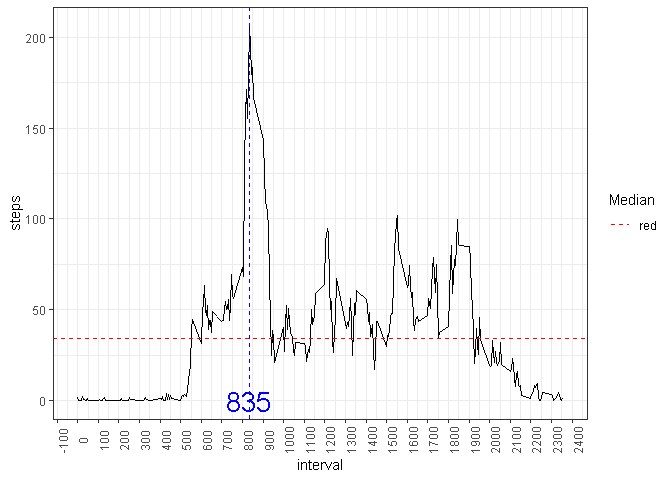
\includegraphics{PA1_template_files/figure-latex/unnamed-chunk-10-1.pdf}

\hypertarget{imputing-missing-values}{%
\subsubsection{Imputing missing values}\label{imputing-missing-values}}

\textbf{Note that there are a number of days/intervals where there are
missing values (coded as \color{red}{\verb|NA|}NA). The presence of
missing days may introduce bias into some calculations or summaries of
the data.}

\begin{itemize}
\tightlist
\item
  Calculate and report the total number of missing values in the dataset
  (i.e.~the total number of rows with
  \color{red}{\verb|NA|}\texttt{NAs}).
\end{itemize}

\begin{Shaded}
\begin{Highlighting}[]
\NormalTok{step6 <-}\StringTok{ }\KeywordTok{table}\NormalTok{(}\KeywordTok{sum}\NormalTok{(}\KeywordTok{is.na}\NormalTok{(csv0)))}
\NormalTok{step7 <-}\StringTok{ }\KeywordTok{data.frame}\NormalTok{(}\StringTok{"NAs Steps"}\NormalTok{=csv0}\OperatorTok{$}\NormalTok{steps, }\StringTok{"NAs dates"}\NormalTok{=csv0}\OperatorTok{$}\NormalTok{date, }\StringTok{"NAs intervals"}\NormalTok{=csv0}\OperatorTok{$}\NormalTok{interval)}
\NormalTok{step7b <-}\StringTok{ }\KeywordTok{data.frame}\NormalTok{(}\KeywordTok{sapply}\NormalTok{(step7,}\ControlFlowTok{function}\NormalTok{ (x) }\KeywordTok{sum}\NormalTok{(}\KeywordTok{is.na}\NormalTok{(x)), }\DataTypeTok{simplify =}\NormalTok{ T)) ; step7b <-}\StringTok{ }\KeywordTok{transpose}\NormalTok{(step7b)}
\KeywordTok{colnames}\NormalTok{(step7b) <-}\StringTok{ }\KeywordTok{c}\NormalTok{(}\StringTok{"NAsSteps"}\NormalTok{, }\StringTok{"NAsDates"}\NormalTok{, }\StringTok{"NAsIntervals"}\NormalTok{)}
\end{Highlighting}
\end{Shaded}

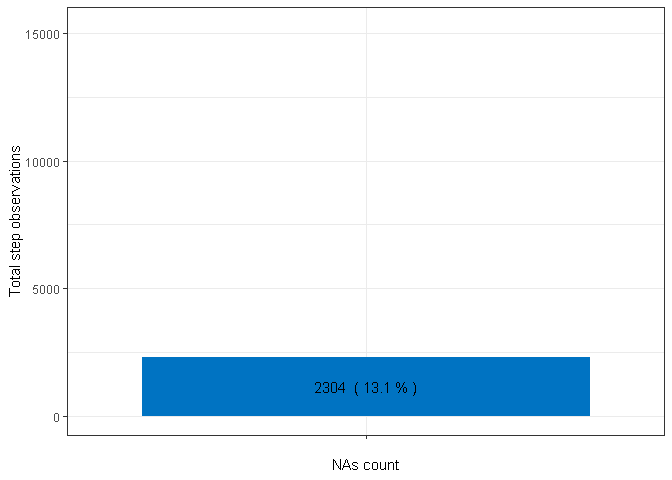
\includegraphics{PA1_template_files/figure-latex/unnamed-chunk-12-1.pdf}

\begin{itemize}
\tightlist
\item
  Devise a strategy for filling in all of the missing values in the
  dataset. The strategy does not need to be sophisticated. For example,
  you could use the mean/median for that day, or the mean for that
  5-minute interval, etc.
\end{itemize}

\begin{Shaded}
\begin{Highlighting}[]
\NormalTok{step8 <-}\StringTok{ }\NormalTok{csv0}
\NormalTok{step8 <-}\StringTok{ }\NormalTok{step8 }\OperatorTok
\StringTok{  }\CommentTok{## Grouping by intervals}
\StringTok{  }\KeywordTok{group_by}\NormalTok{(interval) }\OperatorTok
\StringTok{  }\CommentTok{## Applying grouped mean for each respective NA}
\StringTok{  }\KeywordTok{mutate}\NormalTok{(}\DataTypeTok{steps =} \KeywordTok{ifelse}\NormalTok{(}\KeywordTok{is.na}\NormalTok{(steps), }\KeywordTok{mean}\NormalTok{(steps, }\DataTypeTok{na.rm=}\NormalTok{T), steps))}
  \CommentTok{## Rounding observations as integers}
\NormalTok{step8}\OperatorTok{$}\NormalTok{steps <-}\StringTok{ }\KeywordTok{format}\NormalTok{(}\KeywordTok{round}\NormalTok{(step8}\OperatorTok{$}\NormalTok{steps)); step8}\OperatorTok{$}\NormalTok{steps <-}\StringTok{ }\KeywordTok{as.integer}\NormalTok{(step8}\OperatorTok{$}\NormalTok{steps)}
\end{Highlighting}
\end{Shaded}

\begin{itemize}
\tightlist
\item
  Create a new dataset that is equal to the original dataset but with
  the missing data filled in.
\end{itemize}

\begin{Shaded}
\begin{Highlighting}[]
\NormalTok{step9 <-}\StringTok{ }\KeywordTok{merge}\NormalTok{(csv0, step8, }\DataTypeTok{by =} \KeywordTok{c}\NormalTok{(}\StringTok{"date"}\NormalTok{,}\StringTok{"interval"}\NormalTok{))}
\NormalTok{step9 <-}\StringTok{ }\NormalTok{step9[,}\KeywordTok{c}\NormalTok{(}\DecValTok{1}\NormalTok{,}\DecValTok{2}\NormalTok{,}\DecValTok{4}\NormalTok{)]; }
\KeywordTok{colnames}\NormalTok{(step9) <-}\StringTok{ }\KeywordTok{c}\NormalTok{(}\StringTok{"date"}\NormalTok{,}\StringTok{"interval"}\NormalTok{,}\StringTok{"steps"}\NormalTok{)}
\end{Highlighting}
\end{Shaded}

\begin{itemize}
\tightlist
\item
  Make a histogram of the total number of steps taken each day and
  Calculate and report the mean and median total number of steps taken
  per day.
\end{itemize}

\begin{Shaded}
\begin{Highlighting}[]
\NormalTok{step10 <-}\StringTok{ }\KeywordTok{aggregate}\NormalTok{(steps }\OperatorTok{~}\StringTok{ }\NormalTok{date, }\DataTypeTok{data=}\NormalTok{step9, sum)}
\NormalTok{step10mean <-}\StringTok{ }\KeywordTok{mean}\NormalTok{(step10}\OperatorTok{$}\NormalTok{steps)}
\NormalTok{step10median <-}\StringTok{ }\KeywordTok{median}\NormalTok{(step10}\OperatorTok{$}\NormalTok{steps)}
\end{Highlighting}
\end{Shaded}

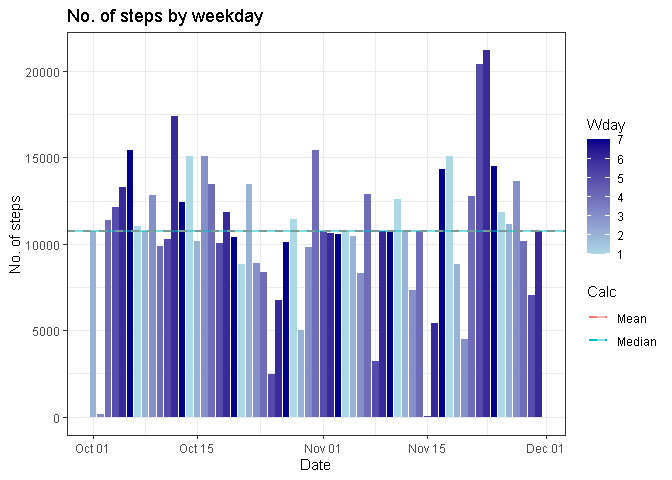
\includegraphics{PA1_template_files/figure-latex/unnamed-chunk-16-1.pdf}

\begin{itemize}
\tightlist
\item
  Do these values differ from the estimates from the first part of the
  assignment? What is the impact of imputing missing data on the
  estimates of the total daily number of steps?
\end{itemize}

Both graphs presents equal values, except for the missing ones, however,
the mean \& median are affected making them similar to each other.

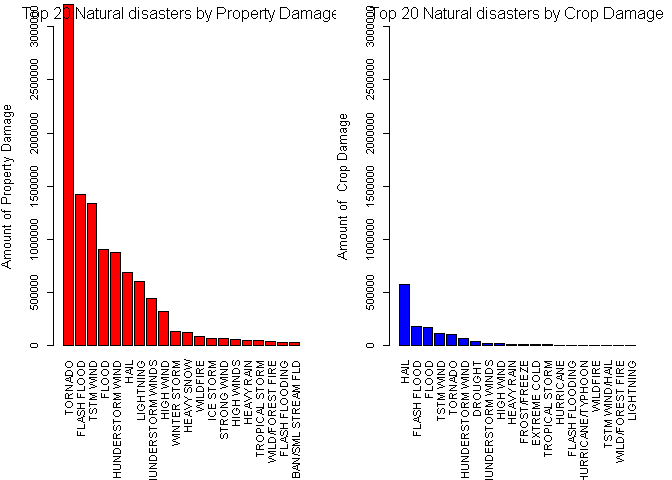
\includegraphics{PA1_template_files/figure-latex/unnamed-chunk-18-1.pdf}

\hypertarget{are-there-differences-in-activity-patterns-between-weekdays-and-weekends}{%
\subsubsection{Are there differences in activity patterns between
weekdays and
weekends?}\label{are-there-differences-in-activity-patterns-between-weekdays-and-weekends}}

\textbf{For this part the \color{red}{\verb|weekdays()|}weekdays()
function may be of some help here. Use the dataset with the filled-in
missing values for this part.}

\begin{itemize}
\tightlist
\item
  Create a new factor variable in the dataset with two levels --
  ``weekday'' and ``weekend'' indicating whether a given date is a
  weekday or weekend day.
\end{itemize}

\begin{Shaded}
\begin{Highlighting}[]
\KeywordTok{Sys.setlocale}\NormalTok{(}\StringTok{"LC_ALL"}\NormalTok{, }\StringTok{"English"}\NormalTok{)}
\end{Highlighting}
\end{Shaded}

\begin{verbatim}
## [1] "LC_COLLATE=English_United States.1252;LC_CTYPE=English_United States.1252;LC_MONETARY=English_United States.1252;LC_NUMERIC=C;LC_TIME=English_United States.1252"
\end{verbatim}

\begin{Shaded}
\begin{Highlighting}[]
\NormalTok{step9}\OperatorTok{$}\NormalTok{wday <-}\StringTok{ }\KeywordTok{ifelse}\NormalTok{(lubridate}\OperatorTok{::}\KeywordTok{wday}\NormalTok{(}\KeywordTok{as.Date}\NormalTok{(step9}\OperatorTok{$}\NormalTok{date), }\DataTypeTok{label=}\NormalTok{T, }\DataTypeTok{abbr=}\NormalTok{T) }\OperatorTok\StringTok{ }\KeywordTok{c}\NormalTok{(}\StringTok{"Sat"}\NormalTok{, }\StringTok{"Sun"}\NormalTok{), }\StringTok{"Weekend"}\NormalTok{, }\StringTok{"Weekday"}\NormalTok{)}
\end{Highlighting}
\end{Shaded}

\begin{itemize}
\tightlist
\item
  Make a panel plot containing a time series plot
  (i.e.~\color{red}{\verb|type = "l"|}\texttt{type\ =\ "l"}) of the
  5-minute interval (x-axis) and the average number of steps taken,
  averaged across all weekday days or weekend days (y-axis). See the
  README file in the GitHub repository to see an example of what this
  plot should look like using simulated data.
\end{itemize}

\begin{Shaded}
\begin{Highlighting}[]
\NormalTok{steptmp <-}\StringTok{ }\KeywordTok{aggregate}\NormalTok{(steps }\OperatorTok{~}\StringTok{ }\NormalTok{interval }\OperatorTok{+}\StringTok{ }\NormalTok{wday, }\DataTypeTok{data=}\NormalTok{step9, mean)}
\end{Highlighting}
\end{Shaded}

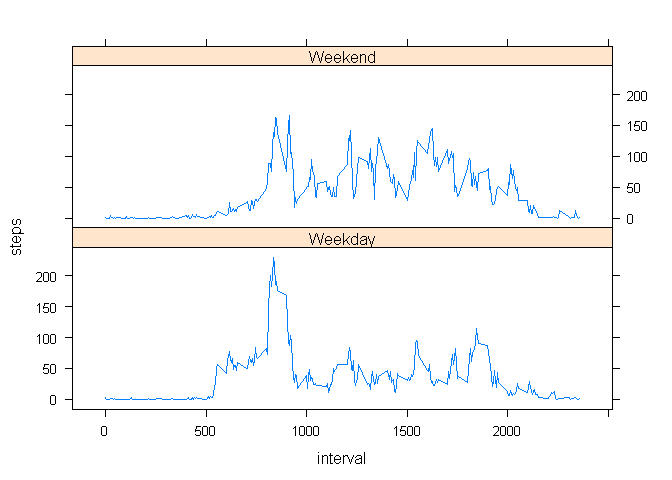
\includegraphics{PA1_template_files/figure-latex/unnamed-chunk-21-1.pdf}

\end{document}
